\documentclass[compress,framenumber]{beamer}

\usetheme{UniversityofCambridge}

\usepackage{lipsum}
\usepackage{natbib}
\newcommand{\nat}{Nature}
\newcommand{\grl}{Geophysical Research Letters}
\newcommand{\gji}{Geophysical Journal International}
\newcommand{\jgr}{Journal of Geophysical Research (Solid Earth)}
\newcommand{\pepi}{Physics of the Earth and Planetary Interiors}
\newcommand{\epsl}{Earth and Planetary Science Letters}
\newcommand{\gca}{Geochimica et Cosmochimica Acta}
\newcommand{\cmp}{Contributions to Mineralogy and Petrology}
\newcommand{\bssa}{Bulletin of the Seismological Society of America}
\newcommand{\toms}{ACM Transactions on Mathematical Software}
\setbeamertemplate{bibliography item}[triangle]

\title{Marsquakes: A key to the structure and history of Mars' deep interior
\\$\,$}
\subtitle{GCB, May 11\textsuperscript{th} 2016}

\author{\hfill{Bob Myhill, Nick Teanby, James Wookey}} 
\begin{document}

% Title page
\begin{frame} 
\titlepage
\vspace{-1.0em}
\end{frame}


\section{Introduction}
% Motivation

\begin{frame}
  \frametitle{Mars: What do we know?}


Use these equations in one of the 'step' slides
\center{$P = \int_{r}^{R} \rho(P, T) g(r') dr' $, $g = 4\pi \frac{G}{r^2} \int_0^r
  \rho(P, T) r'^2 dr'$}
\end{frame}




\section{The InSight Mission}

\begin{frame}
  \frametitle{How do we find this stuff out?}

\end{frame}

\begin{frame}
  \frametitle{Ray paths}
  \vspace{-4.0em}
  \begin{figure}
    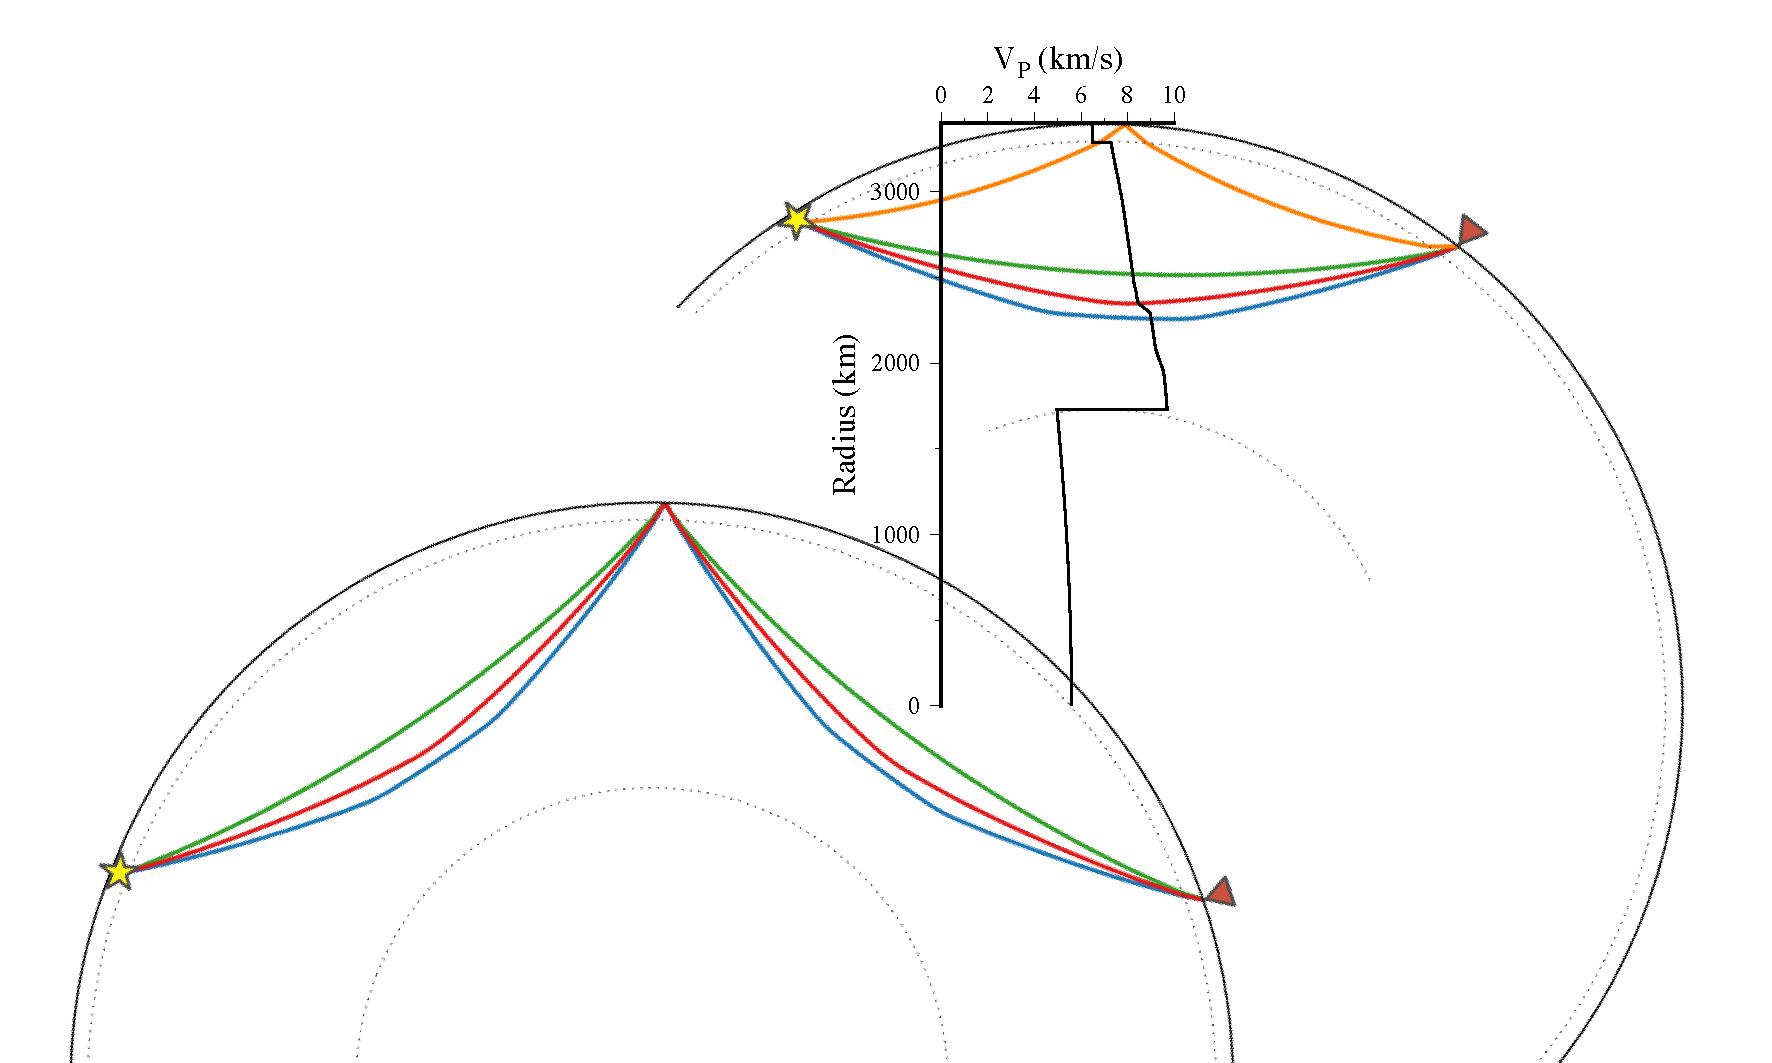
\includegraphics[width=0.95\linewidth]{figures/ray_paths.pdf}
  \end{figure}
\end{frame}

\begin{frame}
  \frametitle{Ray paths}
  \vspace{-4.0em}
  \begin{figure}
    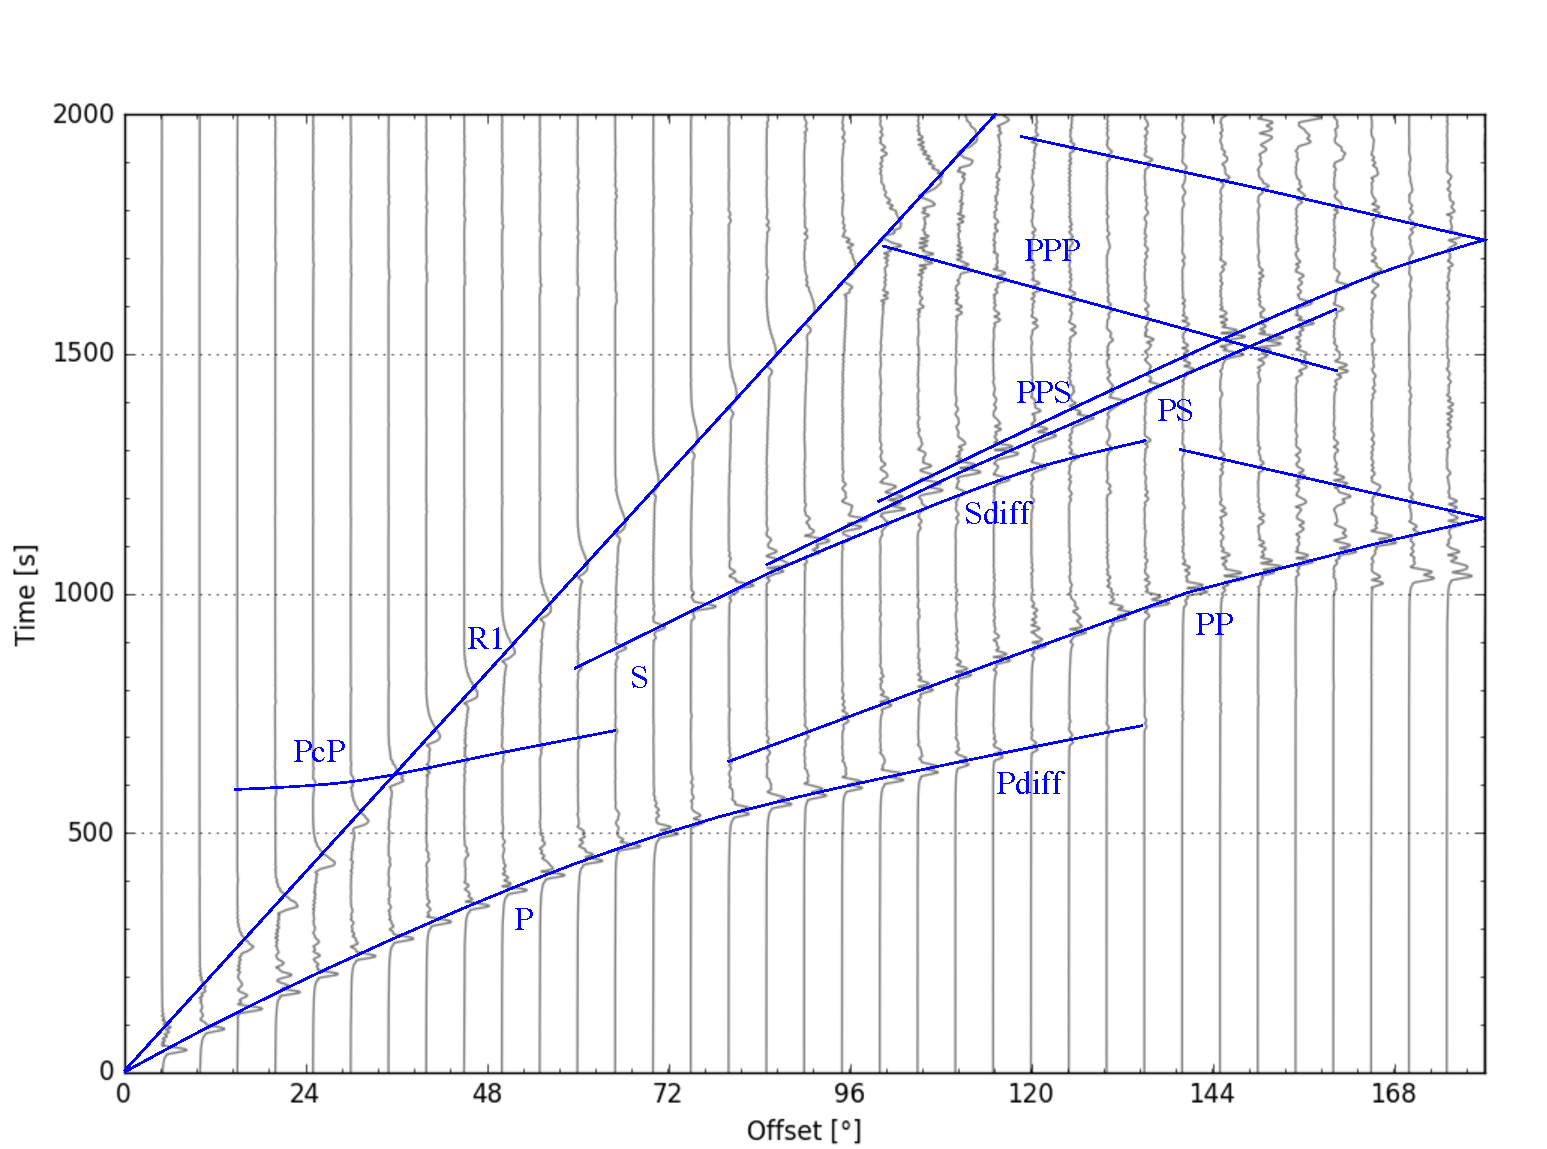
\includegraphics[width=0.95\linewidth]{figures/record_section.pdf}
  \end{figure}
\end{frame}





\end{document}
